The final-state topology in the $t$-channel is characterized by the presence of  exactly one isolated muon and a b jet from the top quark decay, as well as a light-flavour jet produced in the forward region. The splitting of the gluon from the initial state produces a second b quark (Fig. ~\ref{fig:FG}) that recoils against the top quark. The b jet from gluon splitting has generally a softer $p_\mathrm{T}$ spectrum and a broader $|\eta|$ distribution compared to the one produced in top-quark decay, thus the acceptance for events with two b jets reconstructed in the final state is expected to be small. In fact we can anticipate that using the selection described in this section, the number of signal events with two b jets reconstructed in the detector is smaller than the number of events with just one b jet.
Here in the following, we describe the object definitions and selection criteria.


\subsection{Object definition}
\label{sec:objects}

In this Section the basic analysis objects are defined on which the event selection and the kinematic reconstruction are based.
The reconstruction of all objects is done through the PF algorithm~\cite{CMS-PAS-PFT-09-001}. 

 \subsubsection{Tight Muons}
 \label{sec:tight_muon}
 Reconstructed muons within the \texttt{HLT\char`_IsoMu20\char`_eta2p1} trigger acceptance range ($|\eta| < 2.1$) and with a transverse momentum $p_\mathrm{T} >$22~\GeV are selected. The baseline muon selection contains ``global muons'' and has to meet additional muon quality requirements referred to as ``tight muon ID'', which corresponds to a subset of the PF muons. 
 
 More specifically, muons must have $\chi^2/\mathrm{ndof}<10$ and at least one valid hit in the muon chambers, in order to suppress hadronic punch-through and muons from decays in flight. To guarantee a good $p_\mathrm{T}$  measurement, muon candidates are required to have more than 5 valid hits in the silicon tracker, out of which at least one in the pixel detector so as to further suppress muons from decays in flight. At least two segments must match the global muon object in the muon chambers, for suppress punch-through and accidental track-to-segment matches. Furthermore, the (absolute) transverse impact parameter must be smaller than 0.2~cm with respect to the center of the estimated beam spot position in order to suppress the background due to cosmic-ray muons, while the longitudinal distance of the muon track relative to the leading primary vertex\footnote{If more than one primary vertex is identified, the one with largest sum of the squared transverse momenta of associated tracks is taken.} must be less than 0.5~cm at the point of the closest approach.
 
 We define the ``particle flow (relative) isolation'' ($\PFrelIso$) with the so-called ``DeltaBeta'' correction as
 \begin{equation}
 \PFrelIso = \frac{ \pfChargedHadronIso + max((\pfPhotonIso + \pfNeutralHadronIso - \pfPU),0)}{p_T}~,
 \label{eq:pfreliso}
 \end{equation}
 where $\pfChargedHadronIso$, $\pfPhotonIso$, and $\pfNeutralHadronIso$ are the sum of the transverse energies deposited by stable particles like charged hadrons, photons and neutral hadrons respectively, in a cone of size $\Delta R = \sqrt{(\Delta\eta)^2+(\Delta\phi)^2} = 0.4$ around the muon direction; $\pfPU \equiv \Delta\beta \times \sumPUPt \equiv 0.5 \times \sumPUPt$ is the sum of transverse momenta of tracks associated to non-leading, i.e. pileup, vertices, used to estimate the contribution of neutral particles from pileup events by applying a multiplicative factor of 0.5 that takes into account the neutral-to-charged particles ratio expected from isospin invariance. Therefore, the $\Delta\beta$ factor maps the expected neutral contribution in the isolation cone from the observed PU charged contribution. Tight muons are accepted by the requirement $\PFrelIso < 0.06$, which is expected to select signal events with $\sim70\%$ efficiency ($85\%$ corresponds to a cut-value of 0.12, which was used in a former version of the analysis).
 
 Finally, the $\Delta R = \sqrt{\Delta\eta^2+\Delta\phi^2}$ distance must be greater than 0.3 from any jet passing the selection of Sec.~\ref{sec:jets}.
 
 
 
 \subsubsection{Loose Muons}
 
 For the purpose of vetoing events with additional charged leptons, the selection requirements for these additional leptons are loosened. Any event with a further muon, within the full muon acceptance range ($|\eta| < 2.5$), having $p_\mathrm{T} >$~10~\GeV, the ``global'' or the ``tracker muon'' flag (a muon that is reconstructed in the inner tracker and has one segment in the muon chambers) and lying within $\PFrelIso < 0.2$, is rejected. 
 
 
 \subsubsection{Loose Electrons}
 
 The loose electron candidate selection requires a ``GsfElectron'', i.e. electron reconstructed matching a track with the clusters in the calorimeters, with $E_\mathrm{T} > 20\,$\GeV, $|\eta| < 2.5$ and passing a selection chain made by 9 variables and optimized in a cut-based approach. Due to the presence of strong correlation between the  $\Delta\phi$ and $|1/E-1/p|$ (with E the supercluster energy and p the track momentum at the point of closest approach to the beam spot) variables, optimization has been achieved only for one of them, albeit making a reasonable cut for the other. The present analysis then makes use of the cut-based ``electron veto'' working point ($95\%$ signal efficiency) derived using the PHYS14 samples for the PU20bx25 scenario. In addition, the barrel-endcap transition region ($1.44<|\eta|<1.57$) is exluded. Any event with one or more electron candidates as defined above is rejected.
 
 
 \subsubsection{Jets}
 \label{sec:jets}
 
 Jets are reconstructed using the anti-$k_t$ clustering algorithm~\cite{Cacciari:2008gp} with a cone size of 0.4, using the PF algorithm (PF objects as input objects) and after rejecting charged hadrons that are associated to a pileup primary vertex (``slimmedJets''). These jets have standard multi-level (on PU and electronic noise, on $|\eta|$ and on $p_\mathrm{T} >$) jet energy corrections (JEC) applied (L1FastJet, L2, L3) and a $p_\mathrm{T}$ cut at $10\,$\GeV. Technically, we apply the \verb+Summer12+ corrections determined from simulation on both data and simulation.  For data we further apply residual corrections derived from data themselves~\footnote{Label \texttt{Spring10DataV2\_L2L3Residual\_AK5}}. The jet energy is scaled by a factor that describes the detector response depending on the transverse energy and the pseudo-rapidity of the jet~\cite{CMS-PAS-JME-10-003}. To reduce contamination from pileup events, charged particle candidates not associated to the main primary vertex are subtracted event by event. The energy of the jet is then corrected by the amount of energy deposited by neutral pile-up hadrons in the jet area.
 
 The analysis considers jets within $|\eta|<4.7$ whose calibrated transverse energy is greater than 40~\GeV
 and which pass a set of quality cuts (``JET ID'') which are specific of the algorithm used. 
 PF jets must have more than one constituent, neutral hadronic and neutral electro-magnetic energy fractions smaller than 99\%, while their muon fraction should be at most 80\%. In addition, if central, they must have non-zero charged hadronic energy fraction and charged particle multiplicity, whereas their charged electro-magnetic energy fractions must be smaller than 99\%.
 
 Once the jet has been selected according to the above criteria, it is further categorized using a b-tagging discriminator variable 
 in order to distingush between jets stemming from the hadronization of a b-quark or a light parton.

\subsubsection{b Tagging}

Several b-tagging, i.e. identification of jets originating from  b  quarks, algorithms are available in CMS. Some exploit the long B-hadrons lifetime, others their semi-leptonic decay modes and others use kinematic variables related to the high 
B-meson mass and hard b-quark fragmentation function. Details are provided elsewhere~\cite{CMS-PAS-BTV-10-001}. More specifically, b-tagging  algorithms  based  on  displaced  tracks (track counting taggers, jet probability tagger), the presence of ``secondary'' vertices (secondary vertex taggers) or soft leptons (soft lepton taggers) or on a combination of these (combined secondary vertex taggers).  The combined secondary vertex (CSV) taggers combine kinematic variables from displaced tracks and secondary vertices using multivariate analysis (MVA) techniques. Two different taggers are used.  The first makes use of a likelihood ratio (LR), while the second uses a neural network. 
%For this study we use the CSVv2 algorithm at the ``tight'' working point corresponding to a threshold set to 0.941 and a 0.1144\% DUSG mistag efficiency, recomeneded by the The b-tagging Physics Object Group (POG).
For this study we use the CSVv2 algorithm at the ``tight'' working point corresponding to a threshold set to 0.97 and a 0.1\% DUSG mistag efficiency, recomeneded by the The b-tagging Physics Object Group (POG).
%
%\subsubsubsection{pile-up rejection and control-sample specific cuts }
%
%
%After the above cuts are imposed and the jet has been classified according to the b-tagging algorithm, the events are assigned to a specific sample ( see also in the following  Sec-~\ref{sec:leptonjetcounting}). 
%
%Additional cuts are be imposed in the different control regions
%
%For jets failing the b-tagging requirement the root-mean-square radius of the particles with respect to the jet axis ($RMS$) is required to be smaller than 0.025, in order to reject jets from pileup. This requirement is found to improve the agreement of simulation with data in the control regions defined in Sec.~\ref{sec:control}. 
%
%%/An extra cut on the jet $p_T > 60$~\GeV is performed in the signal region in order before performing the fit to extract the inclusive cross section. 
%
%More details will also be given later in this note. 
%%Furthermore, jets of both kinds are ignored if they are within $\Delta R<0.1$ of a tight muon candidate (defined as in Sec.~\ref{sec:tight_muon} apart of course the $\Delta R(\mu,jets)>0.3$ requirement) or $\Delta R<0.3$ of a tight electron candidate (defined as in Sec.~\ref{sec:tight_electron} apart from the requirements on the number of missed hits and photon-conversion veto).
%
\subsubsection{Missing transverse energy}

Defined in an analogous way as PF-based jets, PF-based $\MET$ is the opposite of the vectorial sum of the transverse momenta of the identified PF particles. Data-driven corrections of energy offset are also applied to PF-based \MET. No explicit cut is applied on $\MET$ in this analysis.


\subsection{High level trigger selection}
\label{subsec:hlt}
The offline kinematic thresholds for the prompt muon are imposed by the trigger choice. Therefore a study is performed to evaluate the sensitivity for each trigger requirement. Different single-muon trigger paths are unprescaled for the run range of the analysis of which three are compatible with our kinematics of interest. The \verb+HLT_IsoMu17_eta2p1+ path, imposing $|\eta|<2.1$ on the prompt muon, is the one with the lowest online muon \pt threshold. Other paths are \verb+HLT_IsoMu20_eta2p1+ and \verb+HLT_IsoMu20+ which differ in $\eta$ restriction.

The event selection for this study is exactly the same as that of the signal region, requiring the presence of exactly one prompt muon without any additional loose lepton, two jets of which only one is b-tagged, a W transverse mass above 50 GeV and a top quark candidate with the mass falling in $[130,225]\,\GeV$. The prompt muon selection criteria changes according to the trigger choice. Table~\ref{tab:trigMuSel} summarize the online muon selection with the corresponding offline conditions. The last row is a mixture of the 17 GeV trigger and non-restricted 24 GeV path where a lower offline \pt threshold is applied in $|\eta|<2.1$.

 \begin{table}[t!] 
 \caption{Online muon selection requirements and the corresponding offline conditions}
  \label{tab:trigMuSel}
 \begin{center}
\begin{tabular}{|c|c|}
\hline
Online 	& Offline\\
\hline
\small{HLT\_IsoMu17\_eta2p1 (I)}	& $|\eta|<2.1 ,\, \pt>20\,\GeV$	\\
\small{HLT\_IsoMu20 (II)}			& $|\eta|<2.4 ,\, \pt>22\,\GeV$	\\
\small{HLT\_IsoMu20\_eta2p1} 		& $|\eta|<2.1 ,\, \pt>22\,\GeV$ \\
\small{(I) or (II)}					& $(\pt>20\,\GeV,\,|\eta|<2.1)$ \& $(\pt>22\,\GeV,\,2.1<|\eta|<2.4)$\\
\hline
\end{tabular}
\end{center}
\end{table}

The selection is applied on $t$-channel signal and QCD multijets and $S/\sqrt{B+(\Delta B)^2}$ is taken as a measure for the sensitivity. Table~\ref{tab:hltSensitivity} shows this measure and the yields for different scenarios. The selection corresponding to \verb+HLT_IsoMu20_eta2p1+ seems to have the best performance although the differences are not very significant.

 \begin{table}[t!] 
 \caption{Expected yields and sensitivities at $\mylumi$ for QCD and the $t$-channel signal using different online and offline muon selections. }
  \label{tab:hltSensitivity}
 \begin{center}
\begin{tabular}{|c|c|c|c|}
\hline
Scenario 	& $t$-channel&QCD&$S/\sqrt{B+(\Delta B)^2}$\\
\hline
\small{HLT\_IsoMu17\_eta2p1 (I)}	& $36.6\pm0.99$	&$29.6\pm5.91$	&4.56\\
\small{HLT\_IsoMu20 (II)}			& $35.2\pm0.97$	&$27.2\pm5.67$	&4.57\\
\small{HLT\_IsoMu20\_eta2p1} 		& $36.8\pm0.99$	&$28.4\pm5.79$ 	&4.67\\
\small{(I) or (II)}					& $38.2\pm1.0$	&$30.7\pm6.03$	&4.66\\
\hline
\end{tabular}
\end{center}
\end{table}

Efficiencies for this trigger in data and simulation are obtained using a ``Tag and Probe'' method and details are given in Section \ref{subsec:hlt}. 
%The corresponding data-to-MC correction factors are provided in bins of muon $\pt$, Table~\ref{tab:hltsf}.

% \begin{table}[t!] 
% \caption{The data-to-MC correction factors in bins of muon $\pt$ for the HLT\_IsoMu20\_eta2p1 trigger path.}
%  \label{tab:hltsf}
% \begin{center}
%\begin{tabular}{|l|c|c|c|c|c|}
%\hline
%Bins in muon $\pt$ 	& & & & & \\
%\hline
%Scale factor		& & & & & \\
%\hline
%\end{tabular}
%\end{center}
%\end{table}



\subsection{Lepton counting}
\label{sec:leptoncounting}

As previously described in Sec.~\ref{sec:objects}, we require the presence of exactly one tight muon.
In order to reduce the contribution of dilepton events, which can come from $\ttbar$ or from Drell--Yan processes, 
we veto events with additional loose muons or loose electrons.


\subsection{Jet and b-jet counting}
\label{sec:bcounting}

The signature of the $t$-channel single-top production includes 3 partons in the final state, see Fig.~\ref{fig:FG}(b): 
one light quark recoiling against the virtual W boson, one b quark from the 
top-quark decay, and a second b quark from the initial gluon splitting. 
The second b quark has a softer \pt and a harder $\eta$ spectrum with respect to the one coming from the top-quark decay.
As a result, jets stemming from the hadronization of the latter are less likely to be selected due to the \pt cut on the jet, and if selected they are less likely to be tagged, due to the intrinsic limit on the acceptance in $\eta$ of the b-tagging algorithm, which is limited to the tracker acceptance ($|\eta|<2.5$). For that reason the region with two jets, with one of them being tagged as b jet, provides the largest fraction of signal events. In order to test the modelling of the main background processes it is useful to define further regions, which are enriched in certain background processes. For that purpose we use the notation "nJmT" or the wording "n-jets, m-tags" to refer to a sample that has exactly n reconstructed jets, exactly m of which pass the b tag threshold. Notable samples which are studied and used in this analysis are the 2J0T sample (enriched in \wjets), the 2J1T sample (signal region with the largest signal fraction among all regions), and the 3J2T region (enriched in \ttbar).

%%
%%	\begin{figure}[h]
%%	  \begin{center}
%%            \subfigure[]{
%%            \includegraphics[width=0.48\textwidth]{figures/selection/NBTags_VLightVSTChan_Muons.pdf}} 
%%	    \caption{\label{fig:btag}{	Number of tags with $D_{TCHP} > 3.41$ for data and simulation for signal and \wjets normalized to the same area, after the 2 jets request.  }}
%%	  \end{center}
%%	\end{figure}
%%%Hence we expect most signal events to have only one b-tagged jet. 
%%%&	The highest discriminator value of the high-purity track-counting $b$ tagger in the event is shown in Fig.~\ref{fig:btag}(a), and 
%The b-tag multiplicity in 2-jets events is shown in Fig.~\ref{fig:btag}(a) and~\ref{fig:btag}(c) for data and simulation, 
%and in Fig.~\ref{fig:btag}(b) and ~\ref{fig:btag}(d)
%for signal and W+lf.
%The contribution of processes without b quarks in the final state is strongly suppressed in the 1-tag sub-sample, 
%showing the largest population of signal events at the same time; the small 2-tags sub-sample is dominated by $\ttbar$. 
%Therefore, selected events are required to have exactly one b-tagged jet. 
%%%	\begin{figure}[h]
%%%	  \begin{center}
%%%            \subfigure[]{
%%%            \includegraphics[width=0.48\textwidth]{figures/NBTags_Muons.pdf}}
%%%	    \subfigure[]{
%%%	    \includegraphics[width=0.48\textwidth]{figures/NBTags_Electrons.pdf}}
%%%	    \subfigure[]{
%%%	    \includegraphics[width=0.48\textwidth]{figures/NBTags_VLightVSTChan_Electrons.pdf}}
%%%	    \hfill
%%
%%
%Figure~\ref{fig:nbjetPresel} shows the jet multiplicity after selecting exactly 1 and 2 b-tagged jets, comparing data and MC.
%%
%%Figure~\ref{fig:nbjetPresel} shows the jet multiplicity after selecting exactly 1 and 2 b-tagged jets, comparing data and MC.

%%
%%	\begin{figure}[h]
%%	  \begin{center}
%%	    \subfigure[]{
%%	    \includegraphics[width=0.48\textwidth]{figures/selection/NJetsnJNoPU1TMuStack.pdf}} 
%%	    \subfigure[]{
%%	    \includegraphics[width=0.48\textwidth]{figures/selection/NJetsnJNoPU2TMuStack.pdf}} 
%%%	    \subfigure[]{
%%%            \includegraphics[width=0.48\textwidth]{figures/general/nJEleStack.pdf}}
%%%            \subfigure[]{
%%%            \includegraphics[width=0.48\textwidth]{figures/NJets_TTBarVSTChan_Electrons.pdf}}
%%	    \caption{\label{fig:nbjetPresel}{Jet multiplicity after the lepton counting in data and simulation requiring exactly 1 (a) and 2 (b) jets passing the trackcounting high purity tight threshold.}}
%%	  \end{center}
%%	\end{figure}
%%


\subsection{Transverse W boson mass}
To further suppress contributions from processes where the muon does not come from a leptonically decaying W boson, 
a selection based the reconstructed transverse W-boson mass $\mTW$ is made. The transverse W-boson mass is defined as:  

\begin{equation}
  \mTW = \sqrt{\left(p_{T,l} + p_{T,\nu}\right)^2 
    - \left( p_{x,l} + p_{x,\nu} \right)^2 
    - \left(  p_{y,l} + p_{y,\nu} \right)^2}~,
  \label{eqn:mTW}
\end{equation}
where the transverse momentum components of the neutrino are approximated by the components of the missing transverse energy vector, $\vec\MET$.
Only events with $\mTW > 50\,$\GeV are kept for the analysis.

%
%This variables is used for \qcd rejection in the muon channel. More details on the \qcd treatment can be found in section ~\ref{sec:QCD}
%
%
%%Figure~\ref{fig:mTW} shows the distribution of the $\mTW$ distribution after the preceding selection. 
%%In Fig.~\ref{fig:mTW} the QCD background can be nicely distinguished, since the transverse mass of the alleged W bosons accumulates 
%%at low values while all processes with real W bosons tend to cluster around the W mass
%%(this feature is known in the literature as ``Jacobian peak''). 
%%	Hence, the reconstructed transverse $W$-boson mass is required to be above 50~\GeV for the event to be kept. 
%%
%%
%%	\begin{figure}[h]
%%	  \begin{center}
%%	    \subfigure[]{
%%	      \includegraphics[width=0.48\textwidth]{figures/2j1t/mtwMassMuStack.pdf}}
%%	    \subfigure[]{
%%	      \includegraphics[width=0.48\textwidth]{figures/MTWMass_QCDvsTChan_Muons.pdf}} \\
%%            \subfigure[]{
%%              \includegraphics[width=0.48\textwidth]{figures/2j1t/metPtEleStack.pdf}}
%%           \subfigure[]{
%%              \includegraphics[width=0.48\textwidth]{figures/MET_QCDvsTChan_Electrons.pdf}}
%%            \caption{\label{fig:mTW}{Transverse mass after the entire selection minus the $\mTW$ ($\MET$) cut, 
%%                in data and simulation (a: muons, c: electrons) and for signal and QCD background (b: muons, d: electrons). }}
%%	  \end{center}
%%	\end{figure}	
%%
%%	\begin{figure}[h]
%%	  \begin{center}
%%	    \subfigure[]{
%%	      \includegraphics[width=0.48\textwidth]{figures/mtwMass_WSample_noSyst_MuStack.pdf}}
%%	    \subfigure[]{FIXME
%%	      \includegraphics7~[width=0.3\textwidth]{CMScol}}
%%           \subfigure[]{
%%             \includegraphics[,width=0.48\textwidth]{figures/mtwMass_WSample_noSyst_EleStack.pdf}}
%%	    \subfigure[]{FIXME
%%	      
\includegraphics[width=0.3\textwidth]{CMScol}}
%%          \caption{\label{fig:mTW_nobtag}{Transverse mass after the entire selection minus the $M_T$ in the zero $tche$ tag bin, corresponding to Sample A defined in ~\ref{sec:wjets} (a muons, b electrons).}}%FIXME, and optimization of the threshold (b muons, d electrons).}}
%%	  \end{center}
%%	\end{figure}	
%%
%%, its better stability against variations of the \MET~scale (see Sec.~\ref{sec:syst}), and because \MET~turns out to be quite correlated with muon momentum and muon isolation in our QCD sample, since most of the surviving QCD events in the muon channel, and many also in the electron channel, have a true lepton coming from $b$ or $c$ decay, therefore they also have a true neutrino.
%%Moreover, differently from \MET, the $M_T$ distribution is roughly similar for all non-QCD events, and this permits a very simple way to extract the amount of QCD background from data, as presented in Sec.~\ref{sec:qcd}.
%%In this analysis the $\mTW$ threshold is determined for muons with the following procedure:  
%%a fit to the $\mTW$ distribution is performed as described in Sec.~\ref{sec:qcd} in order to obtain the number of W-like and QCD-like events in the data sample. 
%%The $\mTW$ threshold is then selected maximizing the figure of merit $W/\sqrt{W+Q+(kQ)^2}$, with $k=50\%$, where $W$ ($Q$) is the estimated number of W-like 
%%(QCD-like) events, and which takes into account the total uncertainty on the number of QCD-like events determined in the fit. %More details are given in Appendix~\ref{sec:mt_cut}.
%%The threshold chosen for muons is $\mTW>40$~\GeV , while for electrons it is $\MET>35$~GeV.  
%%
%
%\subsection{\etalj}
%\label{sec:etalj}
%
%
%The distribution of the pseudorapidity $\etalj$  of the recoil from the fragmentation of
%a light quark in the $t$-channel scattering (Fig.~\ref{fig:FG}(c)) extends to value larger than for the background 
%processes, as shown in Fig.~\ref{fig:etalj_mc}.
%
%\begin{figure}[htp]
%\centering
%\includegraphics[angle=00,width=0.48\textwidth]{figures/tChanTTEta.pdf}
%\caption{Pseudorapidity of the untagged jet (\etalj) for the signal after requiring 2 jets 1 tag vs the distribution of the same variable for 
%\tt events, normalized to unity }
%\label{fig:etalj_mc}
%\end{figure}
%
\subsection{Top quark reconstruction}
\label{sec:topreco}

In order to define signal and sideband regions based on the top quark mass and to analyze the kinematics of singly produced top quarks, the fourvector of the top quarks have to be reconstructed from the decay products. All top-quark decay products are reconstructed in the detector, except for the neutrino which escapes unobserved. While the transverse momentum of the neutrino can be inferred from the missing transverse energy, its longitudinal momentum has to be derived based on  extra assumptions. Once the leptonically decaying W boson is reconstructed the selected jets have to be assigned to the final state quarks in the top quark decay chain.

\subsubsection{W-boson reconstruction}
\label{mlbnu}

The first step in the reconstruction of the top quark from its decay products is the reconstruction of the W boson. 
We assume that the $x$ and $y$ components of the missing transverse energy are entirely due to the escaping neutrino, 
and apply the W-mass constraint in order to extract the unknown $z$ component ($p_{z,\nu}$):
\begin{equation}
\label{eq:wconstraint}
\mW^2 = (E_{\ell} + \sqrt{{\MET}^2 + p_{z,\nu}^2})^2 - (\vec p_{T,\ell}+\vec\MET)^2 - (p_{z,\ell}+p_{z,\nu})^2 ~.
\end{equation}

This equation has in general two solutions:
\begin{equation}
\label{eq:solutions}
p_{z,\nu} = \frac{\Lambda \cdot p_{z,\ell}}{p_{T,\ell}^2} 
\pm \sqrt{
\frac{\Lambda^2\cdot p^2_{z,\ell}}{p_{T,\ell}^4} 
- \frac{E^2_{\ell}\cdot {\MET}^2 - \Lambda^2}{p_{T,\ell}^2}
}~,
\end{equation}
with
\begin{equation}
\label{eq:muW}
\Lambda = \frac{\mW^2}{2} + \vec p_{T,\ell}\cdot \vec \MET~.
\end{equation}

In the case of two real solutions for $p_{z,\nu}$ (in $65\%$ of all cases), different choice criteria have been proposed~\cite{Abazov:2009ii, Aaltonen:2009jj}. The solution with the smallest absolute value is chosen in the present analysis. By looking at truth information in simulated events it is found that, in $63.4\%$ of the selected events with real solutions, the smallest $|p_{z,\nu}|$ solution is closer to the true neutrino $p_{z}$ than the other solution. Figure~\ref{fig:pz_solution} shows the diffence in $p_z$ of the reconstructed neutrino with respect to the true neutrino for the cases of choosing the $\min |p_z|$ value, the $\max |p_z|$ value and the closest value amongst the two solutions ($\min \Delta p_{z}$).

\begin{figure}[hbpt]
\begin{center}
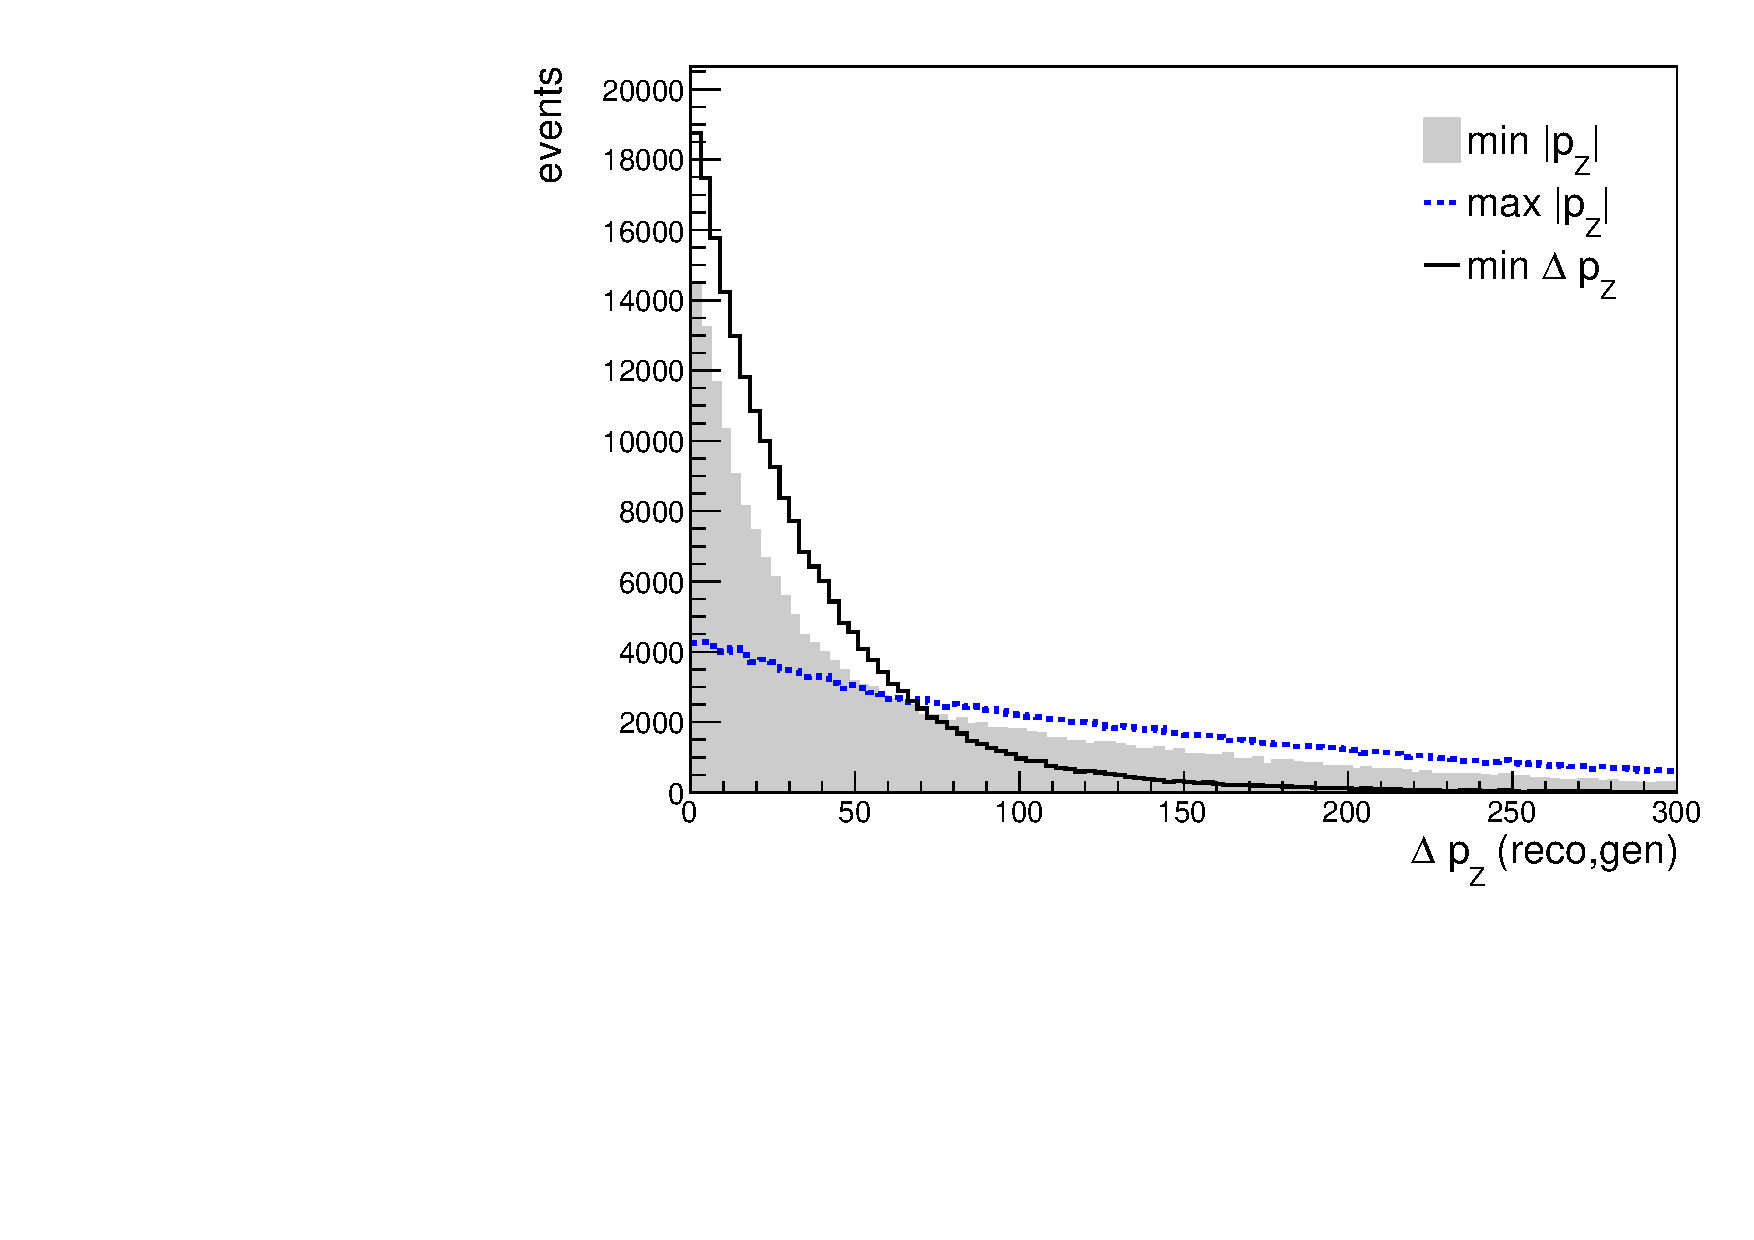
\includegraphics[width=0.6\textwidth]{figures/pz_solution.pdf}
\caption{\label{fig:pz_solution}Comparison of $p_{z}$-solutions against the difference in $p_{z}$ to the true neutrino.}
\end{center}
\end{figure}

If the discriminant in Eq.~(\ref{eq:solutions}) becomes negative, or equivalently $\mTW$ is larger than $\mW$, 
the solutions have an imaginary component. 
This happens in 35\% of the cases, mostly due the finite $\MET$ resolution. Lepton momentum resolution and the finite W intrinsic width give negligible contributions.
Several schemes have been used to deal with this situation~\cite{Abazov:2009ii, Aaltonen:2009jj}. In this analysis the imaginary component is eliminated by modifying $\MET$ such to give $\mTW = \mW$, still respecting the $\mW$ constraing from Eq.~(\ref{eq:wconstraint}). This is obtained by imposing that the discriminator, and thus the square-root term in Eq.~(\ref{eq:solutions}), are null. This condition gives a quadratic relation between 
$p_{x,\nu}$ and $p_{y,\nu}$, with two possible solutions, 
among which the one with minimal distance between $p_{T,\nu}$ and $\MET$ is chosen.


\subsubsection{Jet-parton assignment}

\begin{figure}[hbpt]
\begin{center}
\subfloat[][]{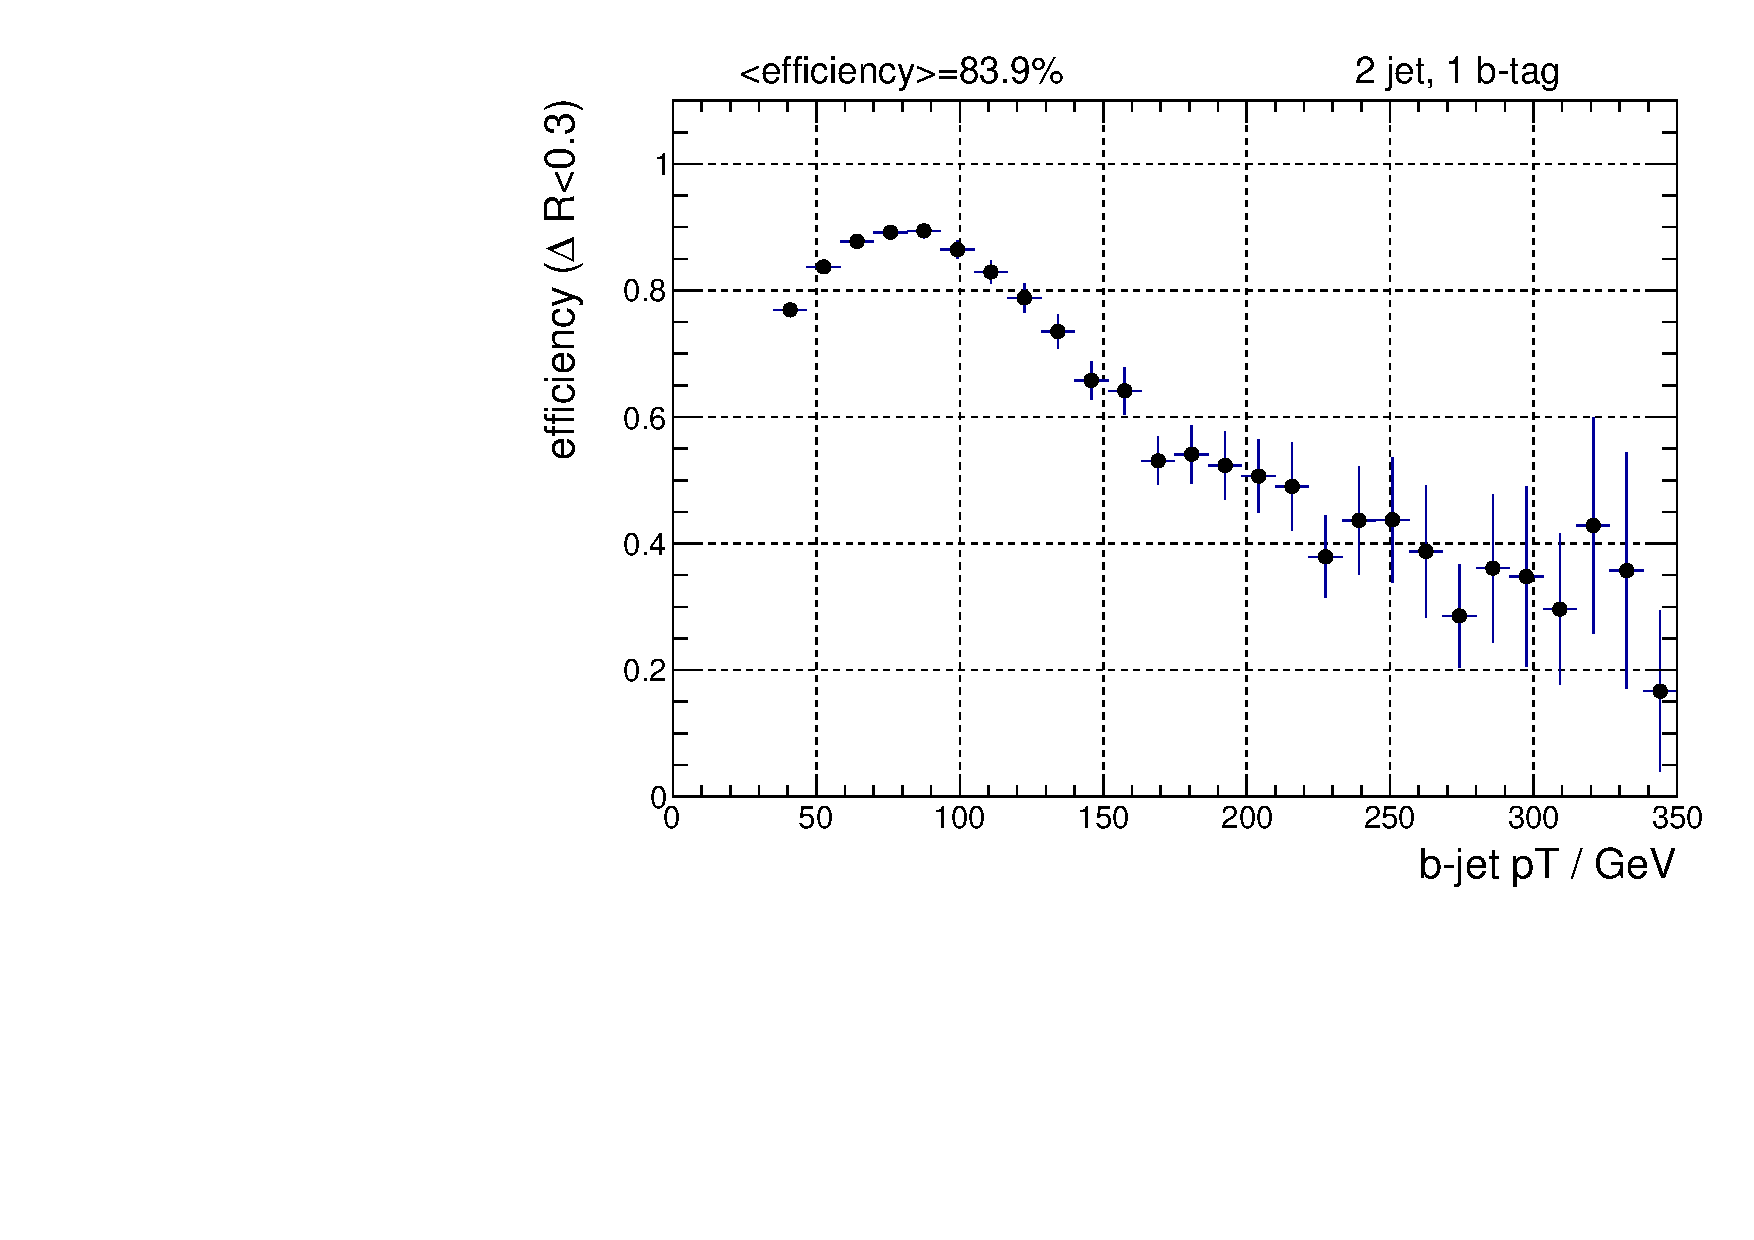
\includegraphics[width=0.45\textwidth]{figures/reconstruction/matching_topdecay_2j1t_pt.pdf}}\hspace{0.05\textwidth}\subfloat[][]{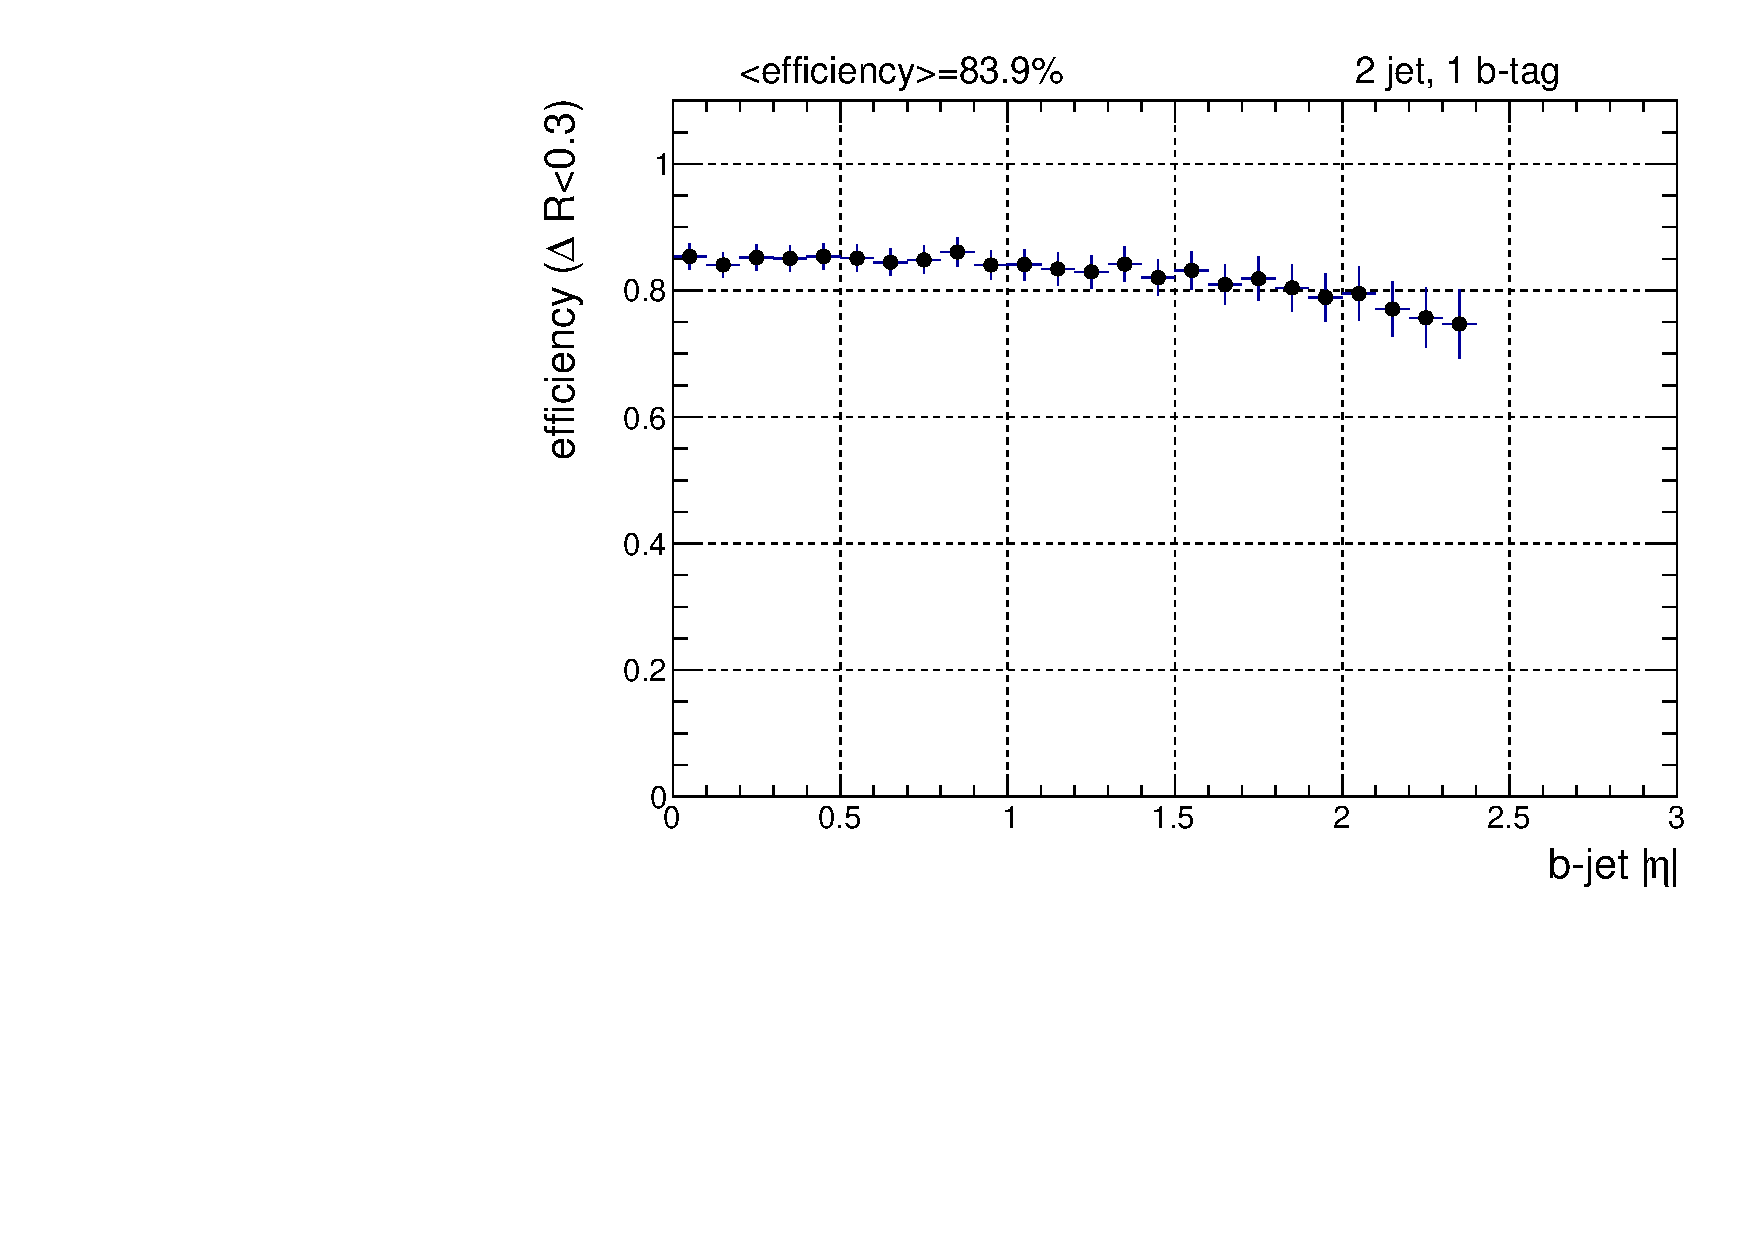
\includegraphics[width=0.45\textwidth]{figures/reconstruction/matching_topdecay_2j1t_eta.pdf}}
\caption{\label{fig:2j1t_matching_bjet_topdecay}Matching efficiencies between the true b-quark from the top decay and the selected tagged jet ($\Delta R<0.3$) in the ``2jet 1tag'' signal region.}
\end{center}
\end{figure}

In the second step the selected jets have to be assigned to the final state quarks from the top-quark decay. In the 2J1T region the procedure is straight forward: the tagged jet is assigned to the b-quark from the top-quark decay, the non-tagged jet is assigned to the light quark. The b-tagged jet matches the true b quark  from top-quark decay in simulated events in about 83.9\% of the selected signal events, using as matching criterion a distance of $\Delta R < 0.3$ between the jet and the parton. The fraction of events with wrong assignmet are events in which the selected b-tagged jet stems from the second b-quark from the initial gluon splitting and not from the decay of the top quark. Figure~\ref{fig:2j1t_matching_bjet_topdecay} shows the matching efficiencies against the transverse momentum and pseudorapidity of the selected jet.


\begin{figure}[hbpt]
\begin{center}
\subfloat[][]{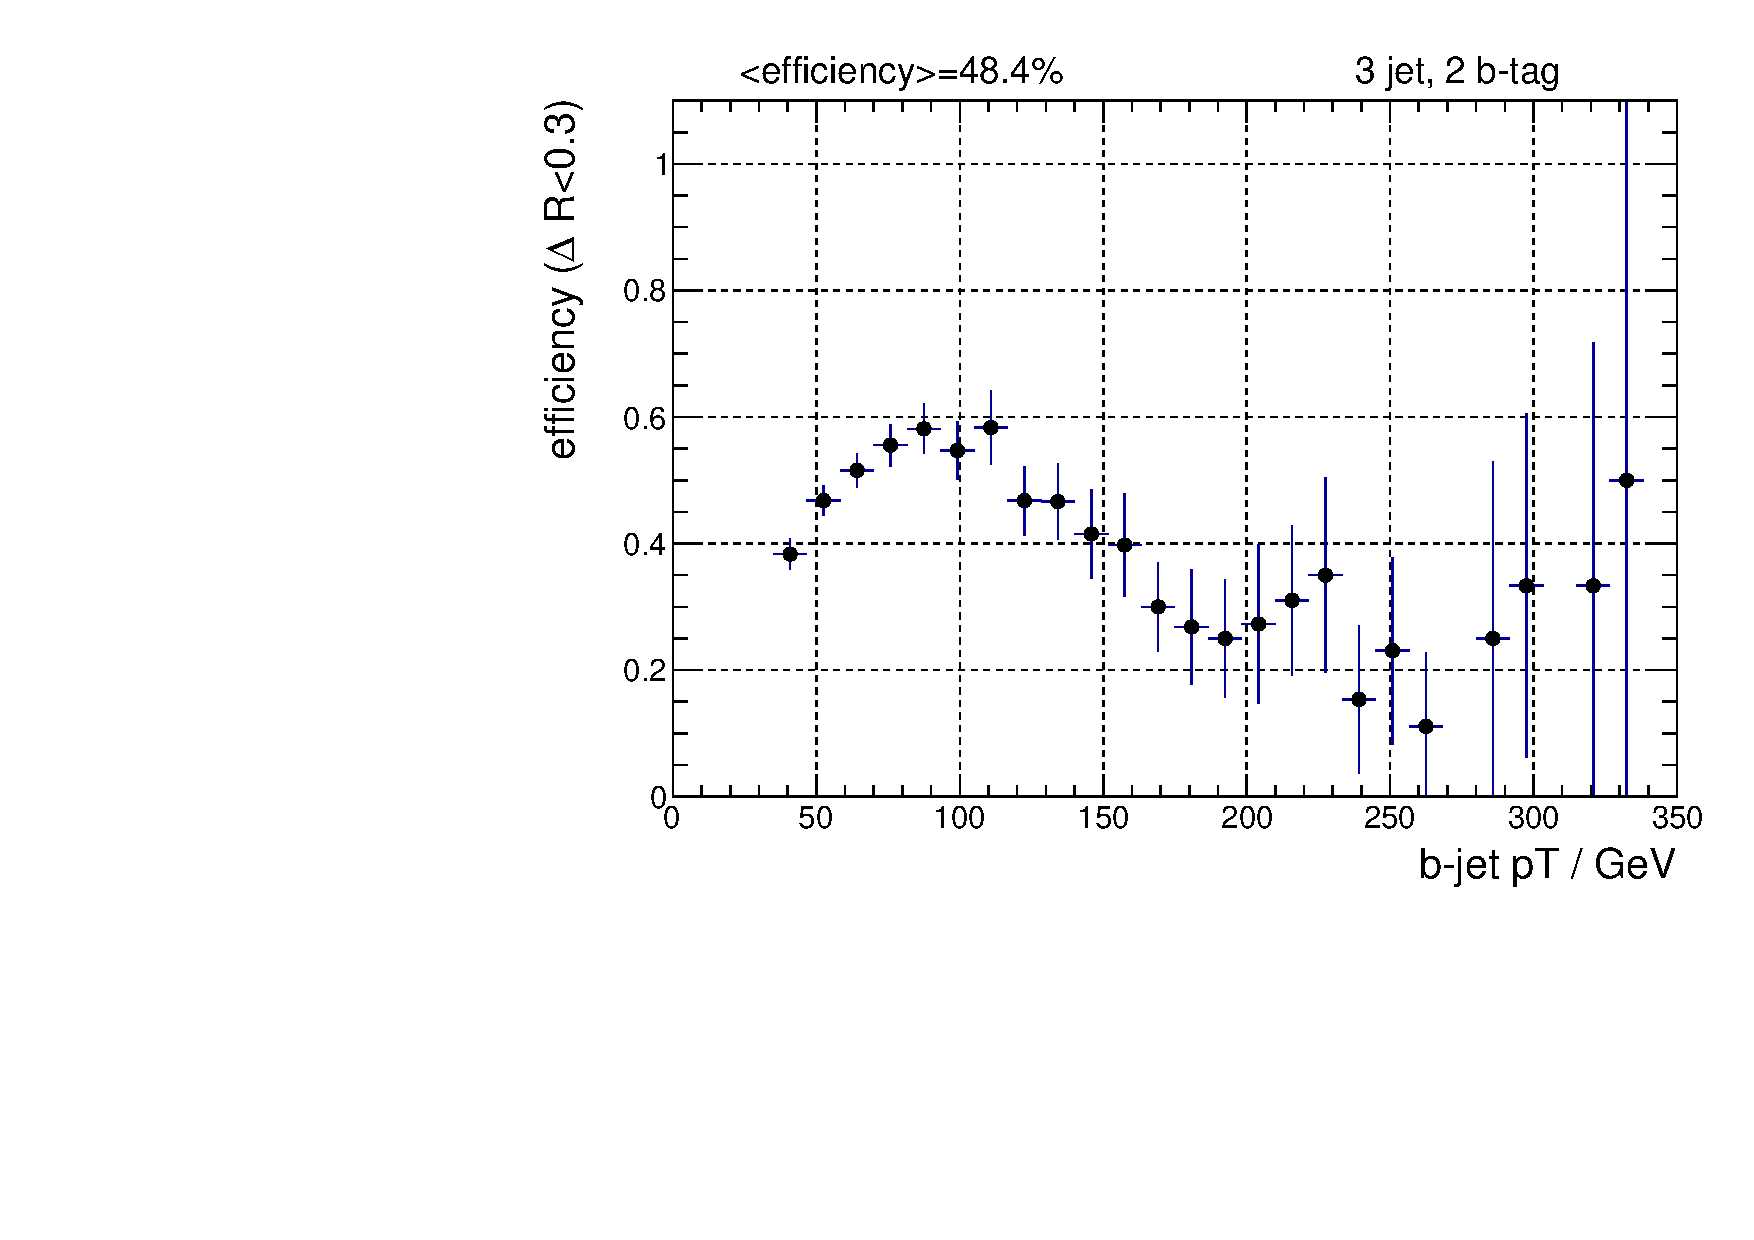
\includegraphics[width=0.45\textwidth]{figures/reconstruction/matching_topdecay_3j2t_pt.pdf}}\hspace{0.05\textwidth}\subfloat[][]{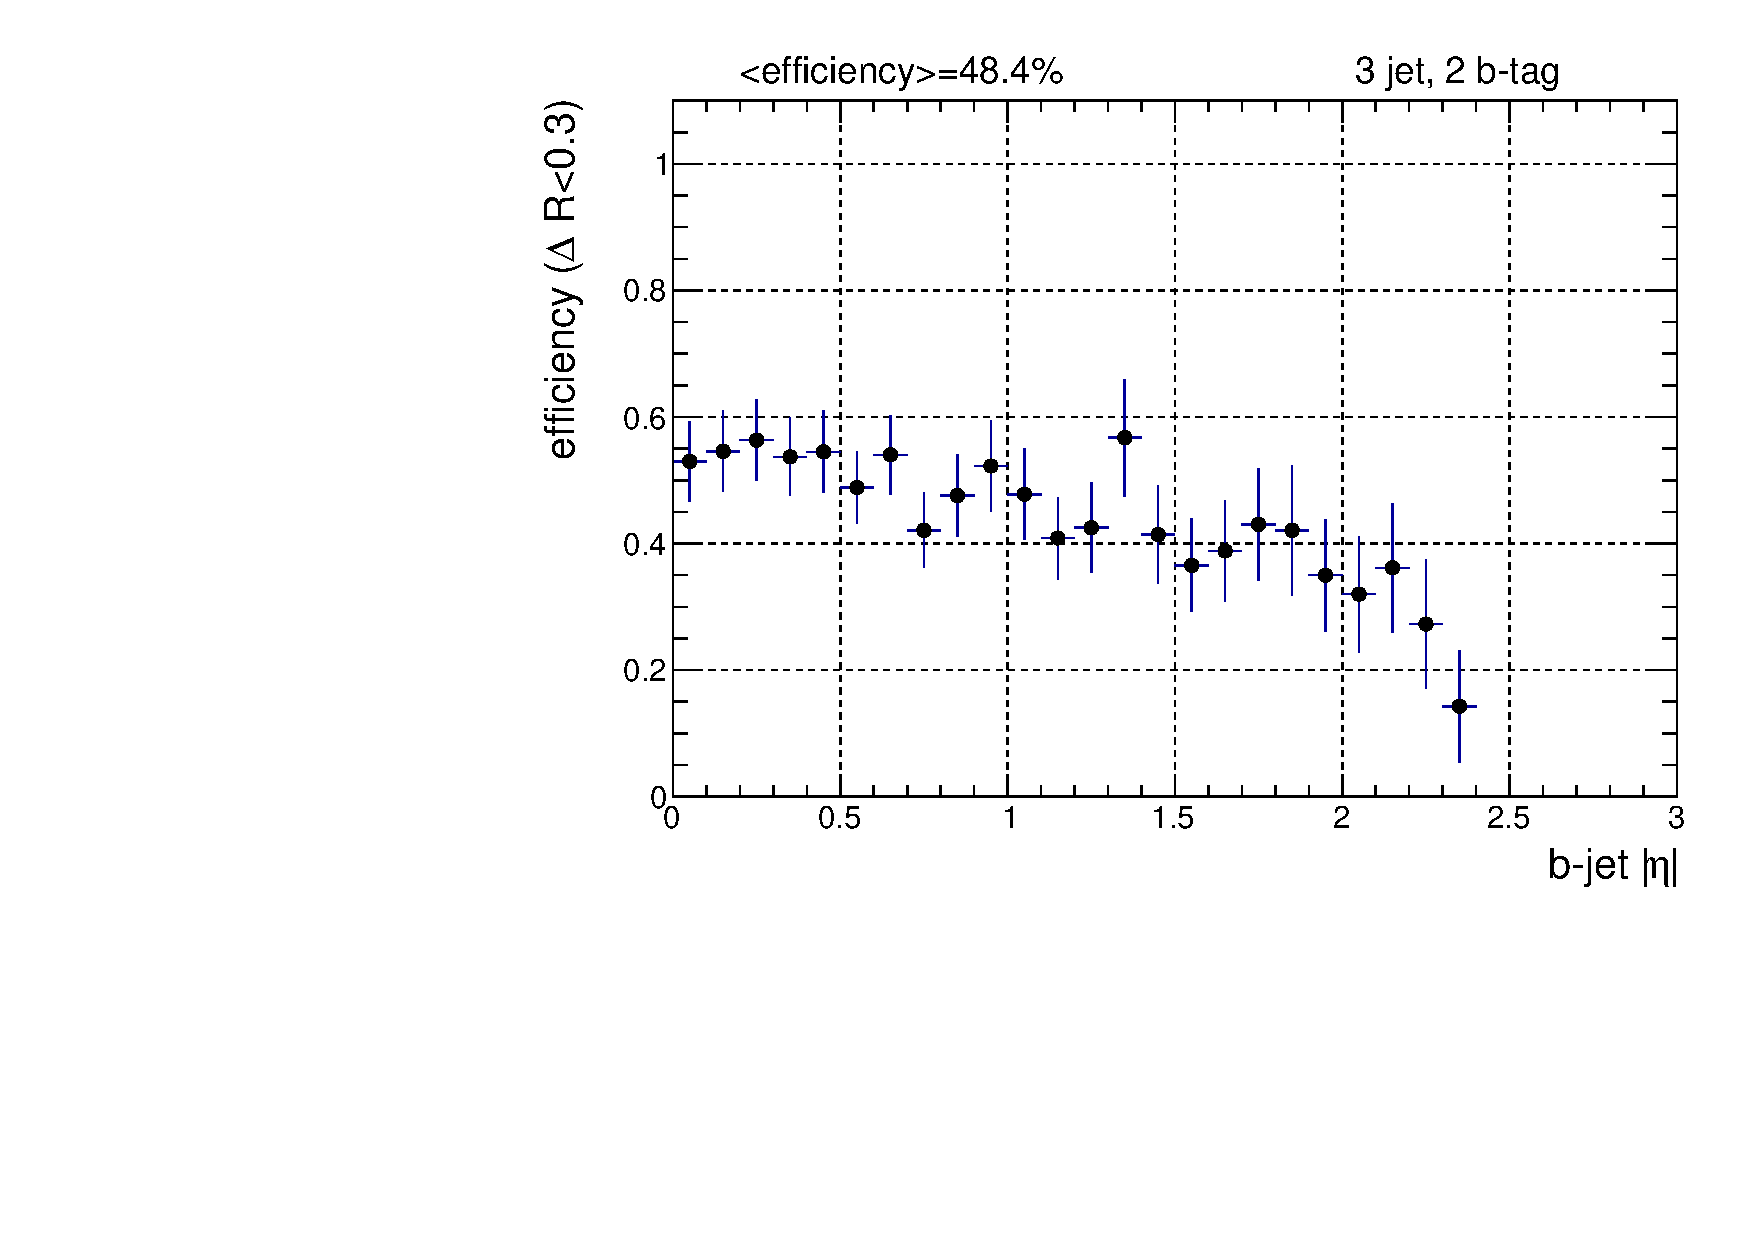
\includegraphics[width=0.45\textwidth]{figures/reconstruction/matching_topdecay_3j2t_eta.pdf}}
\caption{\label{fig:3j2t_matching_bjet_topdecay}Matching efficiencies between the true b-quark from the top decay and the selected tagged jet ($\Delta R<0.3$) in the ``3jet 2tag'' control region.}
\end{center}
\end{figure}


In the 3J2T region the non-tagged jet is again assigned to the light quark. From the two tagged jets the one with the larger value of the b-tag discriminator is assigned to the b quark from the top-quark decay, while the other tagged jet is assigned to the second b quark from the gluon splitting. This choice is correct in 48.4\% of all cases, estimated on simulated signal events using the same matching criterion as described above. The matching efficiencies against the transverse momentum and pseudorapidity of the selected jet are displayed in Fig.~\ref{fig:3j2t_matching_bjet_topdecay}.

          
                
\subsection{Top quark mass cut}

In the signal region (2J1T) we apply an additional cut on the invariant mass of the reconstructed top quark. Events inside the mass window between $130\,$\GeV and $225\,$\GeV are kept while the events outside this region are used to model the background from $\wjets$ (see Sec.~\ref{sec:WHFExtraction}).


\subsection{Event yields}
                
Table~\ref{tab:yields} summarizes the data yield surviving each selection step applied in the current analysis in the signal region 2J1T along with the yields for the signal and various background processes, obtained from MC simulation and scaled to an integrated luminosity of \mylumi. An illustration of table~\ref{tab:yields} is provided in Fig.~\ref{fig:cutflow}.            

\begin{table}[H!] 
 \caption{The number of data events passing each selection step. For comparison also the numbers for the signal and different BG processes are given, obtained from MC simulation and scaled to an integrated luminosity of \mylumi.}
  \label{tab:yields}
 \begin{center}
\begin{tabular}{l|c|c|c|c|c|c|c}
- & QCD & W/Z+Jets &\tt~ and tW & $t$-channel & Sum & Data & Data/MC\\
\hline
Trigger & $3.5\times10^5$ & $4\times10^5$ & 5218 & 616 & $7.5\times10^5$ & 610452 & $79\%$\\
== 1 $\mu$ & $5\times10^4$ & $3\times10^5$ & 3398 & 481 & $3.5\times10^5$ & 318252 & $90\%$\\
== 2 Jets & 2061 & 7962 & 963 & 167 & 11153$\pm$81 & 9509 & $85\%$\\
== 1-bJet & 209 & 127 & 335 & 58 & 729$\pm$18 & 595 & $82\%$\\
$m_T > 50$ & 61 & 88 & 229 & 40 & 418$\pm$11 & 379 & $91\%$\\
$m_{\ell\nu b}$ & 38 & 40 & 157 & 33 & 268$\pm$8 & 252 & $94\%$\\
\end{tabular}
\end{center}
\end{table}


\begin{figure}[H!]
\begin{center}
\subfloat[][]{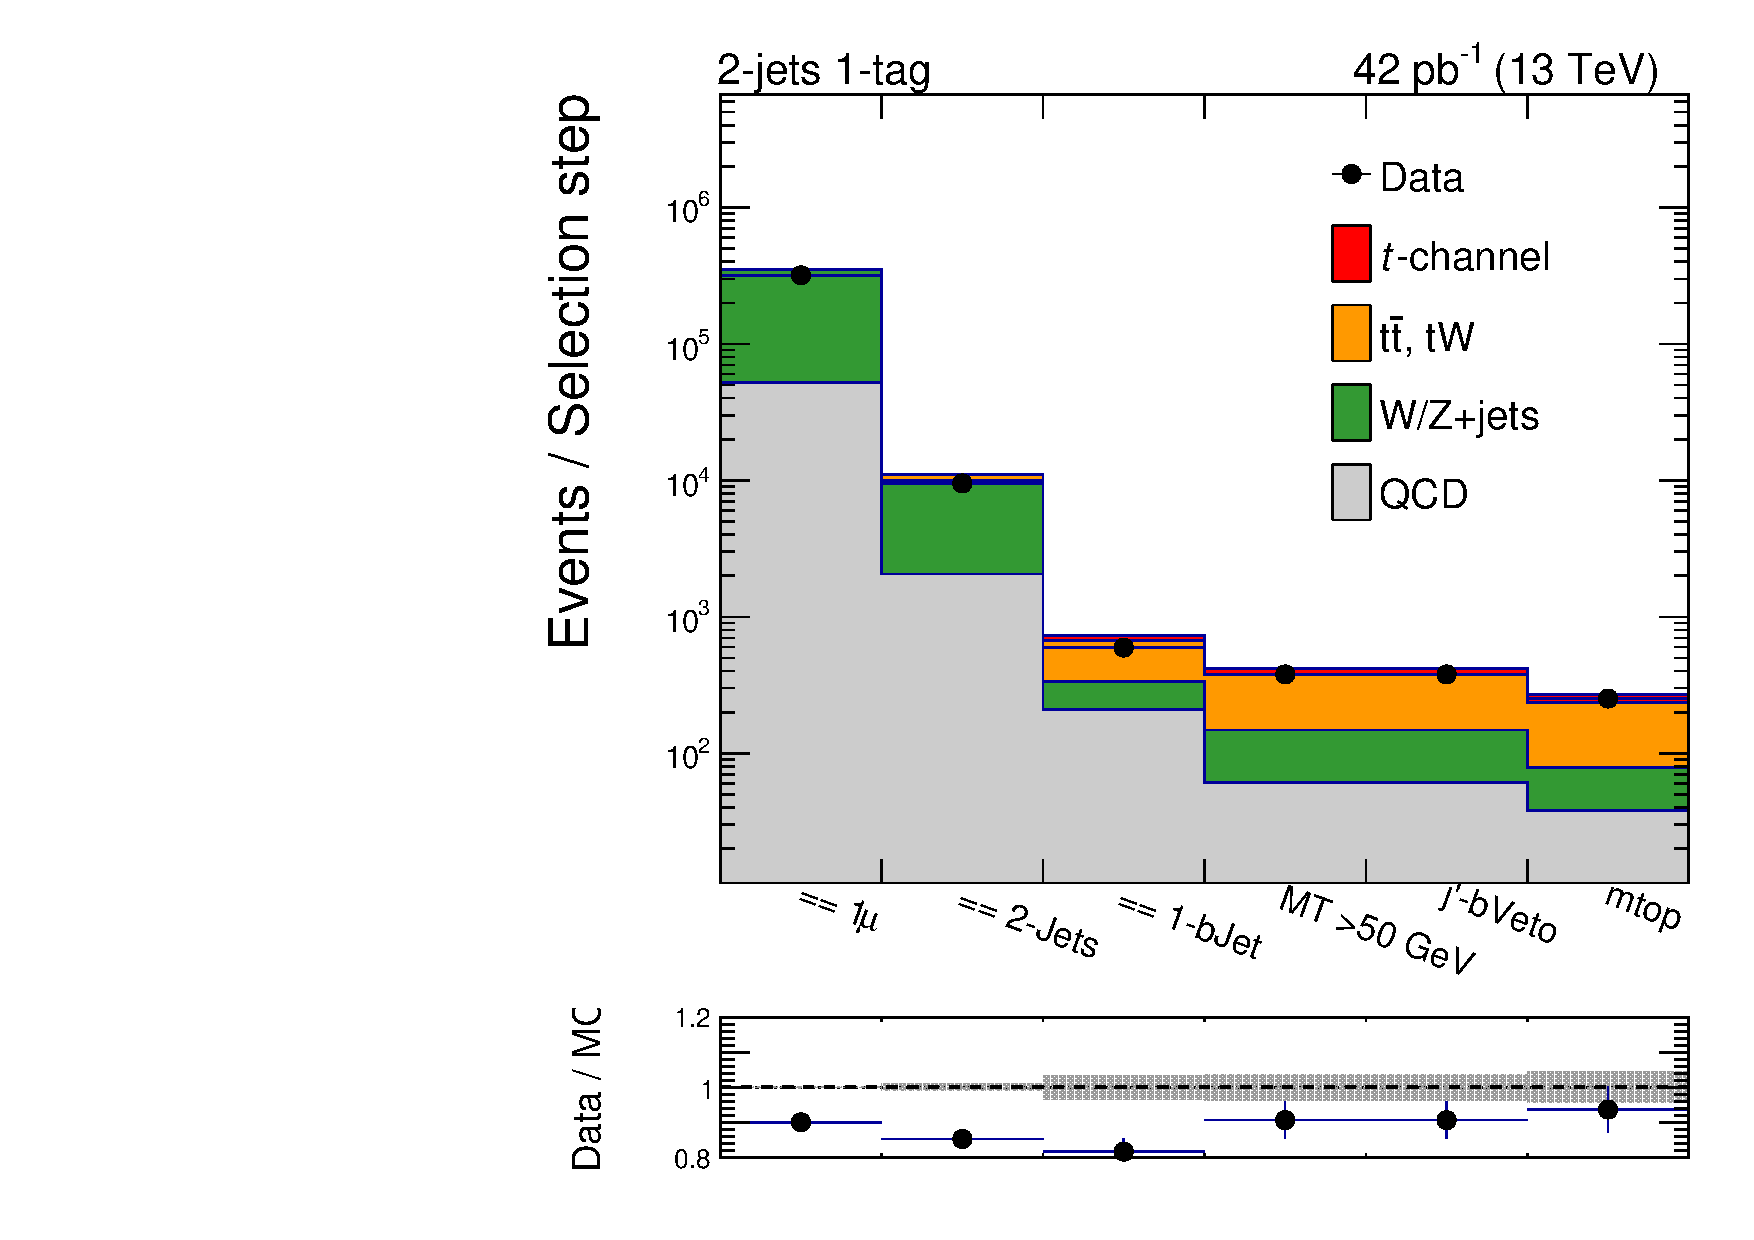
\includegraphics[width=0.6\textwidth]{figures/2J1T/cutflownew.pdf}}
\caption{\label{fig:cutflow}Graphical visualization of the event yields for the different processes after each step of the event selection.}
\end{center}
\end{figure}              
                             
\clearpage

%
%\subsection{Scale factors and reweighting techniques}
%\label{sec:reweighting}
%Scale factors are associated to the selected events in simulation to keep into account further differences between data and MC.
%
%\subsubsection*{Scale factors for b-tagging and mistagging from data}
%\label{sec:btagSF}
%
%Estimates of the selection efficiencies of true and misidentified b-jets 
%can be found in Ref.~\cite{CMS-PAS-BTV-11-004}, as a function of $p_T$ and $\eta$ of the jet.
%Performances are computed for the tight TCHP working point used in this analysis.
%To correct the mistag rates and b-tagging efficiency in simulation each event is weighted by appropriate scale factors, following the procedure explained in Ref.~\cite{rizzi_sf}.
%
%
%\subsubsection*{Pile-up scale factors from data}
%\label{sec:PileUpSF}
%
%One way of evaluating the effect of the PU on the analysis, taking into account the different PU conditions
%during the data taking period, is to determine
%scale factors between the data and simulation. These factors are obtained according 
%to CMS prescriptions: the distribution of the number of true interaction vertices is measured on data, while the 
%same distribution in simulation is known. For each simulated event appropriate weights are applied 
%as a function of the number of interaction vertices, in order to reproduce the distribution of 
%the number of interaction vertices in data (details in Ref.~\cite{pileup_rew}).
%%An example of the true vertices distributions in data and MC is given in Figure ~\ref{fig:truePUEvents}(a),(b) respectively,
%%while Fig.~\ref{fig:truePUEvents}(c),(d) show respectively the the reweighting function obtained from the two and the final 
%%reweighted true distribution function. 
%%
%%It has to be noted that the distribution of weights in Fig.~\ref{fig:truePUEvents}(c) depends on the simulated sample and from the 
%%selection applied, but its average for each sample/selection  is order of 1 with variations of few percents($20\%$ max.).
%%However by construction the weights for events with different pile up multiplicities can differ by as much as 1 or even 2 orders of magnitude.
%%
%%	\begin{figure}[h]
%%	  \begin{center}
%%	    \subfigure[]{
%%	    \includegraphics[width=0.48\textwidth]{figures/selection/PileUpData.png}}
%%	    \subfigure[]{
%%	    \includegraphics[width=0.48\textwidth]{figures/selection/pileUpMC.png}}
%%            \vskip 0.5cm
%%	    \subfigure[]{
%%	    \includegraphics[width=0.48\textwidth]{figures/selection/PileUpWeights.png}}
%%	    \subfigure[]{
%%	    \includegraphics[width=0.48\textwidth]{figures/selection/pileUpRescale.png}}
%%	    \caption{\label{fig:truePUEvents}{True pile up event distribution for data (a), MC(b), rescale function (c) and MC rescaled to data(d).}}
%%	  \end{center}
%%	\end{figure}
%%
%%This can result in the distortion of the shapes of distributions due to the presence of spikes. This effect is more prominent in samples with 
%%low statistics, as shown in figure Fig.~\ref{fig:badcaseexample} and it has potential to be dangerous for samples with higher statistics as well,
%%since it depends on the content of each bin and it is very difficult to keep under control. 
%%
%%The sensitivity of the main variables of this analysis to the pile up, in particular for jets in high pseudorapidity regions, 
%%is first of all studied in the control samples, as it is shown in Sec.~\ref{sec:wjets}. The cuts $p_T>60$~GeV for the two leading jets and $RMS < 0.025$ for the untagged jets are introduced to reduce this sensitivity 
%%and keep the shapes of the variables under control as a baseline strategy.
%%
%%Our strategy for mitigating the effect of the pile up is discussed in the following chapters, in particular Sec.~\ref{sec:wjets}. 
%%%%FIXME:whenever we add it,we uncomment it 
%%%%Section~\ref{sec:pileUp} is dedicated to our strategy for mitigating the pileup effects. 
%%
%%	\begin{figure}[h]
%%	  \begin{center}
%%	    \subfigure[]{
%%	    \includegraphics[width=0.48\textwidth]{figures/selection/3J_1TleptonPtWithPUMuStack.png}}
%%	    \subfigure[]{
%%	    \includegraphics[width=0.48\textwidth]{figures/selection/3J_1TleptonPtNoPUAfterCutsSR_PUWPMuStack.png}}
%%	    \caption{\label{fig:badcaseexample}{Example of reweighted distribution where the spikes due to pile up reweighting alter the shape in
%%	    an unphysical way: muon \pt in the sample where 3 jets ($p_T > 40$~GeV, no $RMS$ cut) are required, one of which b-tagged with (a) and without (b) pile up reweighting, normalized to data yield.}}
%%	    \end{center}
%%	\end{figure}
%%
%%
%%
%%This can be understood looking at the distribution of number of vertices of data and simulation: looking at figure ~\ref{fig:PUs} one can qualitatively expect that 
%%events in regions where data-MC distributions of number of vertices don't overlap will have a low weight and vice versa for events in overlapping regions.
%% Figure~\ref{fig:PUFuncs} confirms this, showing that most of the events in the MC samples have small weights due to the fact that they are in non-overlapping
%%regions in number of vertices. 
%%Those figures refer to two different MC distributions, the one in Figg.~\ref{fig:PUs}(b),~\ref{fig:PUFuncs}(b) having an overall better match with data.
%%
%%Therefore a solution we adopt is to use an overall scale factor for samples with a distribution like those in Figg.~\ref{fig:PUs}(a),~\ref{fig:PUFuncs}(a), 
%%and an event-by-event scale factor for samples with a distribution like those in Figg.~\ref{fig:PUs}(b),~\ref{fig:PUFuncs}(b). 
%%
%%The former is taken sample by sample as the average of the pile up weights of all events composing that sample, and it is always very close to 1 as expected.
%%
%%	\begin{figure}[h]
%%	  \begin{center}
%%	    \subfigure[]{
%%	    \includegraphics[width=0.48\textwidth]{figures/selection/DataVsSummer12PU.png}}
%%	    \subfigure[]{
%%	    \includegraphics[width=0.48\textwidth]{figures/selection/DataVsSummer12V6PU.png}}
%%	    \caption{\label{fig:PUs}{MC (red continuous line) vs data (blue dots) distributions of number of true pile up interactions. 
%%The MC distribution in (a) refers to the ``PU-S7'' production, while (b) refers to the ``PU-S6'' distribution, both described in ~\cite{PUPVTPage}.}}
%%	    \end{center}
%%	\end{figure}
%%
%%
%%	\begin{figure}[h]
%%	  \begin{center}
%%	    \subfigure[]{
%%	    \includegraphics[width=0.48\textwidth]{figures/selection/PUWeight_vs_nVertices.png}}
%%	    \subfigure[]{
%%	    \includegraphics[width=0.48\textwidth]{figures/selection/PUWeight_vs_nVertices_TTBar.png}}
%%	    \caption{\label{fig:PUFuncs}{2D plot of pile up weight vs number of true pile up interactions, mapping Monte Carlo distribution
%%	    to data distributions shown in Fig. ~\ref{fig:PUs}. }}
%%	    \end{center}
%%	\end{figure}
%
